\documentclass[a4paper]{article}
\usepackage{ctex}
\usepackage[left=1.5cm, right=1.5cm, top=1.5cm, bottom=1.5cm]{geometry} %页边距
\usepackage{helvet}
\usepackage{amsmath, amsfonts, amssymb} % 数学公式、符号
\usepackage[english]{babel}
\usepackage{graphicx}   % 图片
%\usepackage{url}        % 超链接
\usepackage{bm}         % 加粗方程字体
\usepackage{multirow}
\usepackage{booktabs}
\usepackage{tikz}%调用宏包tikz
\usepackage{circuitikz}%调用宏包circuitikz
\usepackage{enumerate}
\usepackage{algorithm}
\usepackage{algorithmicx}
\usepackage{algpseudocode}
\usepackage{graphicx}
\usepackage[hidelinks]{hyperref}
\usepackage{listings}
\usepackage{textcomp}
\usepackage{multicol}
\usepackage[backend=biber,style=numeric,sorting=none]{biblatex}
\usepackage{setspace}
%\addbibresource{reference.bib}

% Python listing
\newcommand\pythonstyle{\lstset{
language=Python,
basicstyle=\sffamily,
keywordstyle=\textbf,
commentstyle=\color{blue},
showstringspaces=false, 
numbers=left }}
% Python environment
\lstnewenvironment{python}[1][]{
\pythonstyle \lstset{#1} }{}
\hypersetup{hidelinks,
	colorlinks=true,
	allcolors=blue,
	pdfstartview=Fit,
	breaklinks=true
    }
\newcommand{\threemetrics}[3]{\multirow{3}{*}{\shortstack[c]{$\textcolor{orange}{#1}$\\$\textcolor{blue}{#2}$\\$\textcolor{green}{#3}$}}}
\newcommand{\twometrics}[2]{\multirow{2}{*}{\shortstack[c]{$\textcolor{blue}{#1}$\\$\textcolor{green}{#2}$}}}

\renewcommand{\algorithmicrequire}{ \textbf{Input:}}       
\renewcommand{\algorithmicensure}{ \textbf{Output:}} 
%算法格式
\usepackage{subfigure}
\usepackage{fancyhdr} %设置页眉、页脚
\usepackage{gensymb}

\pagestyle{fancy}
\lhead{Digital signal processing}
\chead{}
\rhead{2024,Homework 3}
\lfoot{}
\cfoot{\thepage}
\rfoot{}
\linespread{2}

\usepackage{ifthen}
\usepackage{xifthen}

\newcommand{\dom}[1]{\mathop{\mathrm{dom}}\left(#1\right)}
\newcommand{\rng}[1]{\mathop{\mathrm{rng}}\left(#1\right)}
\newcommand{\preimg}[2][]{ \ifthenelse{\isempty{#1}}
    {\mathop{\mathrm{preimage}}\left(#2\right)}
    {\mathop{\mathrm{preimage}}_{#1}\left(#2\right)} }
\newcommand{\set}[1]{\left\{#1\right\}}

\newenvironment{proof}{{\par\noindent\it Proof.}\quad\par}{\hfill $\square$\par}
\begin{document}
\section{ReLU 函数的实现}
ReLU 函数的实现通过直接赋值实现。定义线网输入与寄存器输出,我们可以得到ReLU函数的直接实现。\\
\centerline{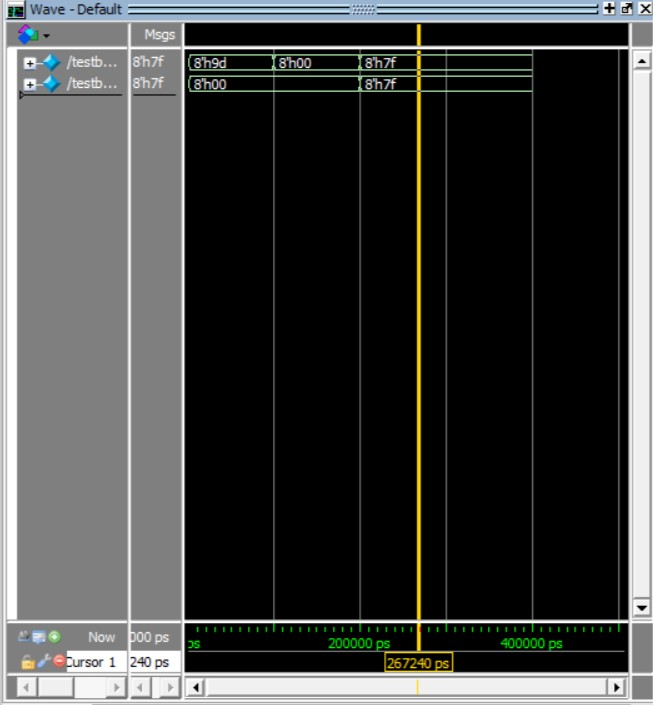
\includegraphics[scale=1.0]{relu.jpg}}\\
图中可以发现,当输入小于等于零时,仿真波形输出为0. 大于零时输出与输入相同。
\section{SiLU 函数的实现}
SiLU函数的表达式为$f(x)=\dfrac{x}{1+e^{-x}}$,因此在Verilog语言中,我们采用线性逼近的方式近似实现
SiLU函数。通过查表法实现。实现波形如下:
\clearpage
\centerline{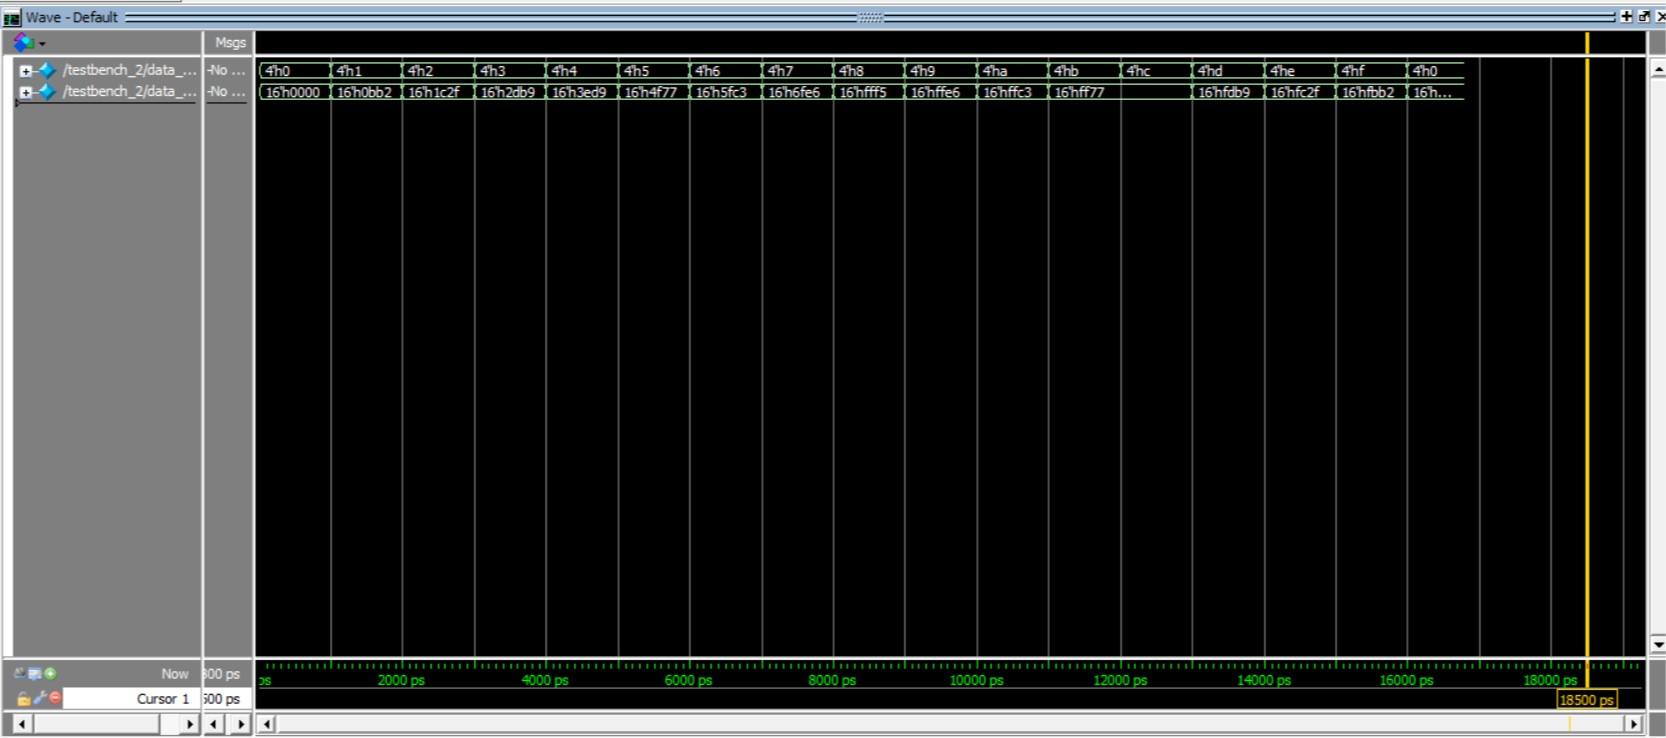
\includegraphics[scale=0.5]{silu.jpg}}
可以看到,该波形符合线性逼近。
\section{SiLU函数多位宽线性插值}
1. 在同学的帮助下,我们发现需要明确输入,中间和输出信号的符号性。默认为无符号型的数将会出现运算(乘法)的问题。\\
2. 首先,我们规定16位,24位和8位的变量。最后过程的乘法可能会出现溢出问题,因此我们采用24位存储。\\
3. 其次,在处理过程中,我们将数字拓展到16位。具体的操作为:(1)将数存储到24位寄存器变量中。由于存储的特性为
高位补0,而我们的中间变量应该仅应该拓展小数位而非整数位。因此将输入数据左移8位。\\
4. 接着,采用移位的方法来实现乘法的功能。具体的方式请参照代码。而不同函数情况的界定,也将其表示成4位整数位和12
位小数位组合而成的16位变量进行划分,从而实现不同的功能。\\
5. 在实现操作前,我们将输入数据绝对值化,即探测寄存器最高位(符号位)是否为1. 随后在最后得到结果后再判断是否需要
输出$1-f(\left|x\right|)$.\\
\centerline{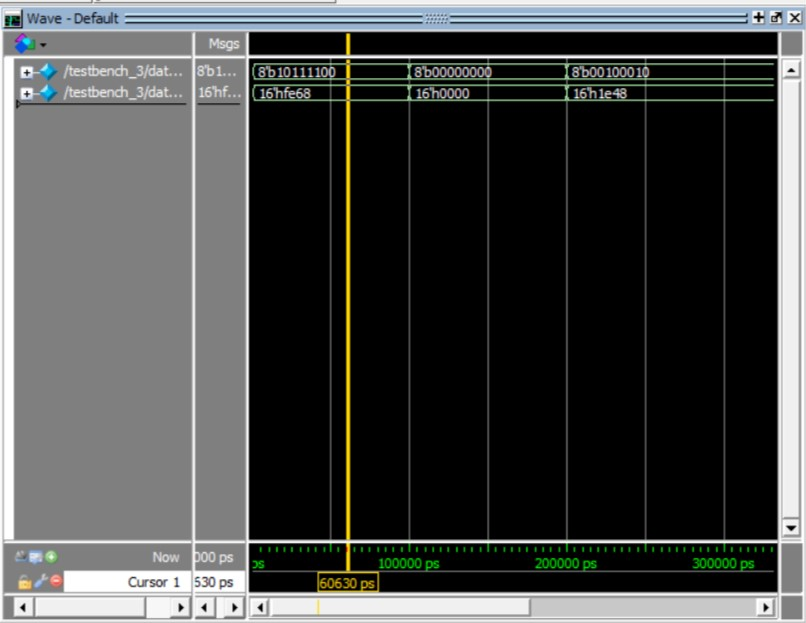
\includegraphics[scale=0.8]{silu_adv.jpg}}
\end{document}